\section{Evaluation}
\label{sec:evaluation}

We evaluated our model in two ways; at the construct level through applying structural equation modeling to a dataset of projects for which security is a concern, and at the SPEF framework level by conducting two case studies of open source development projects, examining the effects of security practice use on security outcomes. In this section, we present a summary description of our case study protocol, SP-EF, and how we apply it to our data collection and analysis. SP-EF and all study artifacts are available online ~\cite{morrison2016spef}. 

\subsection{Quantitative Study Methodology}

To quantitatively assess the relationships between constructs in our proposed model, we applied Structural Equation Modeling~\cite{kline2015principles} to the Core Infrastructure Initiative~\cite{lf2016cii} (CII) census dataset (~\footnote{\url{https://github.com/linuxfoundation/cii-census}}). 

\subsubsection{Structural Equation Modeling}

Kline~\cite{kline2015principles} emphasizes that the point of SEM is to test a theory by specifying a model that represents predictions of that theory among plausible constructs measured with appropriate observed variables (those that can be directly measured). Latent variables represent plausible constructs, e.g. ‘intelligence’, or ‘Criticality’, that cannot be directly measured, but that can be indirectly measured in terms of one or more observed variables. SEM is often applied in psychology and education, to build a measurement model for the constructs measured, and to allow assessment of how well measurement instruments test the constructs measured. 

SEM studies are organized around six steps: specification, identification, data selection and collection, estimation, re-specification, and reporting. In model specification, researchers express the hypothesized relationships between observed variables and latent variables, typically in the form of a graphical model. Each edge in the graph represents a parameter to be estimated, indicating the strength of the relationship between the nodes connected by the edge. In identification, the specified model is checked against statistical theory for whether all of the model’s parameters can be estimated. If the original model cannot be identified, it must be revised in light of both statistical theory and the theory the researcher is expressing in the model. In data selection and collection, data for each of the model’s observed variables is chosen, and collected. In estimation, the observed data and the model are checked for fit.  If appropriate fit is achieved, the parameter estimates can be interpreted for implications of the theorized relationships and the observed data. If appropriate fit is not achieved, the list of model changes developed during specification should be considered in re-specifying the model.  When reporting the results of SEM studies, the model, parameter estimates, and fit measures should be included in the report.
Examples of SEM use in software engineering and information technology include Capra et al.~\cite{capra2008empirical}, Wallace and Sheetz~\cite{wallace2014adoption}, and Gopal et al.~\cite{gopal2005impact}.

\subsubsection{Specification}
For causal hypotheses, we used the hypotheses for each construct in Section \ref{sec:model} to create edges in the model specifying each element’s effect on security risk, practice adherence, and security outcomes.  We model security risk, security effort, and security outcomes as latent variables, explanatory entities that reflect a continuum that is not directly observable~\cite{kline2015principles}. In SEM, latent variables are represented in diagrams as ovals or circles.

\subsubsection{Identification}
In identification, the specified model is checked against statistical theory for whether all of the models parameters can be estimated. Identification is analogous to checking whether a set of equations is solvable given their structure and the data at hand.  Our construct model contains no feedback loops making it both recursive, and, therefore, identified, by Rule 7.1 of Kline ~\cite{kline2015principles}.  

\subsubsection{Data selection and collection}

Kline ~\cite{kline2015principles} states that SEM is a large-sample technique, reporting median sample size in the literature of 200 cases.  Factors that drive the need for a large sample include the size and complexity of the model to be estimated, non-normally distributed data, categorical data, and imprecisely measured data. To obtain a sufficient sample, we draw our study data from summaries of repository data. In particular, we chose the CII census dataset
	because: collects a subset of our constructs, 
We applied the Boa [44] language infrastructure to the full September 2015 Github dataset ro collect project summaries for 68,035 Java language projects We operationalize practice adherence by counting references to each practice’s keywords in commit messages. 

To identify a practice, we adapt Ernst and Mylopoulos’s [28] technique of labeling events in project history, though we measure security practice use rather than requirements discussions, and we use the SP-EF keywords, listed in Table 1, rather than drawing from the ISO 9126 quality model. 

We developed a Boa job  that scans Boa datasets for projects, and produces a single-line summary for each project, including the project name, url, Source Lines of Code (SLOC), number of developers (Devs), references to ‘CVE-‘ records, and keyword counts for each of the security practices and the ‘Security-Related’ keywords.  

To exclude toy projects, we limited the results to those projects with two or more developers, and 1000 or more lines of code.  Because Boa only stores source code information for Java projects, our results include only Java projects. We operationalize security outcomes by counting references to CVE’s in commit messages.  We identified 121 unique projects with one or more CVE’s. 

We randomly sampled 121 projects with no CVE’s from the remaining projects to form a data set of 242 projects.
We were not able to obtain all SP-EF measurements from the repositories. 

To compensate, we kept the structural model intact and adapted or removed some elements of the measurement model to account for the data available from our data sources. 

We now list the adaptations. Since all projects are written in Java, we elided language from the model. 

We removed domain, number of identities, CR, IR, and AR because any selection process we could develop to set values for the variables would add noise to the data. Because of the nature of commit logs, we assume that each unique email address associated with the commit is for a developer. We use the number of developers (‘Devs’), as a proxy for team size. As a proxy for number of machines, we used the number of Google  search results for each repository, reasoning that the search result counts – how widely known the project is - is proportional to how widely used the project is We use counts of CVE references as a proxy for total public vulnerabilities (pre- and post-release), and we calculate VDensity. We do not have a breakdown of when vulnerabilities were discovered for each project, and so we do not measure Pre-Release Vulnerabilities, Post-Release Vulnerabilities, and we do not calculate their ratio, VRE. We use the CVE count and VDensity as our measures of security outcomes. 



\subsubsection{Estimation}
\subsubsection{Re-specification}
\subsubsection{Reporting}


\subsection{Qualitative Case Study Methodology}
In this section, we present a summary description of our case study protocol, SP-EF, and how we apply it to our data collection and analysis. SP-EF and all study artifacts are available online ~\cite{morrison2016spef}. 

Williams et al. ~\cite{williams2004toward} proposed the Extreme Programming Evaluation Framework (XP-EF), a set of repeatable measures for assessing the degree to which a team held to XP practices enabling replication and meta-analysis of studies. We emulate the organization and intent of XP-EF in the construction of SP-EF, while adapting the content to focus on security practice adherence rather than Extreme Programming. SP-EF provides guidelines for data collection of context factors, practice adherence metrics, and outcome measures. Context factors characterize the project by, for example, its size and purpose. Practice adherence metrics are a means of characterizing the degree to which a practice is used on a project. SP-EF includes objective and subjective metrics for measuring practice adherence. Outcome measures characterize the software's security performance. Table \ref{tab:paComparisonTable} lists the SP-EF practices.  
% \ref{fig:fig_context} presents an overview of the SP-EF practices and their place in the software development lifecycle.

%\begin{figure*}
%	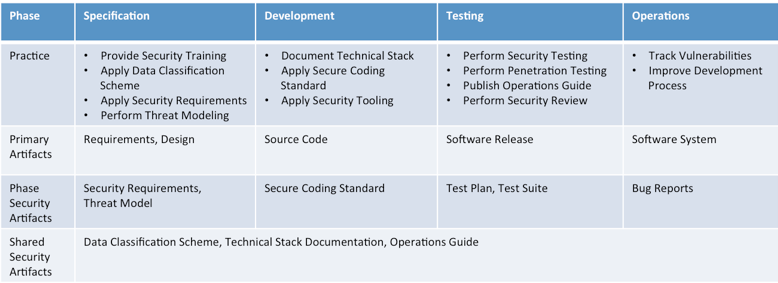
\includegraphics[width=7in]{figure/PracticesDiagram.png}
%	\caption{SP-EF Software Development Security Practices}
%	\label{fig:fig_practices}
%\end{figure*}

To assess our data collection methods and to increase confidence in our findings, we triangulate, collecting data in three ways; through qualitative observation, survey, and text mining of the team's issue tracker. We worked with the project staff and read through the project documentation for qualitative evidence of the security practices, based on the SP-EF subjective practice adherence measures. We conducted a survey of the team, using the SP-EF practice adherence survey. The survey contains demographic questions (e.g. role, time on project), four questions aligned with the SP-EF subjective measures for each SP-EF security practice, and open-ended questions allowing survey participants to express their views. Each of the four subjective adherence measures are actionable; comparing observed results with expected results can be translated to actions for each measure in the following ways;
\begin{itemize}
	\item Usage - ``How often is this practice applied?'' - Lower than expected usage can be addressed by discussing, or requiring, higher frequency of use with the team.
	\item Ease Of Use -``This practice is easy to use'' - Lower than expected Ease of Use can be addressed through, for example, examination and refactoring of work practices, and through training.
	\item Utility - ``This practice assists in preventing or removing security vulnerabilities in our product'' - Lower than expected Utility can be addressed through examining practice use, and, possibly, discontinuing use of the practice.
	\item Training - ``I have been trained in the use of this practice'' - Low training for a practice can be addressed through increasing the availability of training.
\end{itemize}

We piloted the survey within the research group, and with researchers at two companies. The survey questionnaire is available from the SP-EF website. We obtained objective SP-EF practice adherence measures for the team by applying a basic text mining technique, keyword counting, to the project's issue tracking records. The text mining classification procedure is available as an R package, linked from the SPEF website~\cite{morrison2016spef}.   To develop an oracle for assessing the performance of the text mining, we read and classified the set of issue tracking records described above according to the guidelines for identifying the presence of SP-EF practices. We compute recall and precision for the mined objective measures, compared to the manual oracle. 

\subsection{Subject Selection}
We select projects for this study based upon meeting the following criteria:
\begin{itemize}
	
	\item Available records of software security vulnerabilities
	\item Version control system access, providing both project source code and the history of changes to the code over time
	\item Bug tracker system access, providing records of vulnerability and defect discovery and resolution
	\item Project documentation, providing access to information about the project’s development process and practices
\end{itemize}

We collect project documentation and history using the project’s website, version control system, and bug tracker, as primary sources, and as sources for links to further information. 

For this study, we chose OpenSSL, to evaluate security practice use before and after the Heartbleed bug.  For comparison across cases, we choose phpMyAdmin, an open source project of similar age and size to OpenSSL, allowing comparison of how security practices and outcomes are similar and different between the projects. 

\subsection{Data Collection}

We collect data through qualitative observation and text mining of the team's emails, issue tracker, and commit messages. We read through the project documentation for qualitative evidence of the security practices, based on the SP-EF subjective practice adherence measures. We obtained objective SP-EF practice adherence measures for the team by applying a basic text mining technique, keyword counting, to the project's issue tracking records. The text mining classification procedure is available as an R package, linked from the SP-EF website~\cite{morrison2016spef}.   To develop an oracle for assessing the performance of the text mining, we read and classified a subset of the emails, issue tracking records, and commit messages described above according to the guidelines for identifying the presence of SP-EF practices. 

For each practice, we used the search strings listed in the ‘Keywords’ column of Table 1, and recorded each instance of practice use.  We collected data by two means:
\begin{itemize}
	\item We used a script, available from the SP-EF website, to iterate over each commit, issue, and email, and generate security practice event classifications.
	\item The first author manually examined each project for security practice use and generated security practice event classifications. Additional raters classified a randomly selected pool of issues, and we compared their results to the automated classifications.
\end{itemize}

For each artifact we identified, we recorded the document name, URL, age, and made note of any available change history, e.g. wiki page change records. We manually classified pre- and post-release vulnerabilities based on a study of who reported the vulnerability and whether they were identifiable as a project member.

\subsection{Analysis}

We qualitatively compare pre-security event data with post-security event data for each project, looking for changes in the security practices selected by the team, and changes in frequency of use of the practices by the team. In the case of OpenSSL, we manually classified 500 commits, bug tracking issues, and emails from the year before April 1, 2014 (Heartbleed), and 500 more from the year ending April 1, 2016.  We chose the earlier time period to reflect pre-Heartbleed efforts, and the more recent time period to reflect ongoing practice rather than the immediate response to Heartbleed. In the case of phpMyAdmin, we chose the year 2007, reflecting phpMyAdmin data before its participation in GSOC, and from the year ending April 1, 2016, reflecting current practice. By comparing the data sets, we expect to find security-focused practice changes in the text of the sets of project data.

To evaluate RQ1, we collect frequency metrics through manual review of each project’s artifacts; project documentation, project emails, bug tracking issues, and commit messages.  

To evaluate RQ2, we track two outcome measures, counts of CVE and Security-Related (SR) events. CVE's are publicly reported vulnerability counts, which may understate the total vulnerability count.  SR events are counts of references to a set of keyword that represent those found in typical discussions of security, acting as a proxy for the team's awareness of security. Lower values for CVE and SR may indicate high code quality and/or opportunities for discovering latent vulnerabilities. We examine the relationship between our practice adherence metrics and CVE and SR.
